\chapter{Hardware-Based Speculation}
\label{ch:hardware_speculation}

In high-performance microarchitectures, dynamic scheduling alone (such as Scoreboarding or basic Tomasulo's algorithm) cannot extract maximum \gls{ilp} because instruction issue stalls at control flow boundaries (conditional branches). Hardware-based speculation extends dynamic scheduling by fetching, issuing, and executing instructions past unresolved branch conditions, guessing the branch outcome using branch prediction mechanisms and proceeding as if the prediction were correct.

While speculative execution eliminates branch prediction stalls, it necessitates hardware mechanisms to handle mispredictions gracefully. If a branch guess turns out to be incorrect, all speculatively executed instructions along the wrong path must be purged without altering the architectural state. Consequently, speculation introduces a strict requirement: bypassing computed results for execution must be decoupled from the actual architectural completion (commit) of instructions.

\begin{definition}{Hardware-Based Speculation}{hardware-speculation}
    Hardware speculation is a dynamic execution technique where the processor predicts control flow paths and speculatively executes instructions beyond unresolved branches. Speculative instruction outputs can be forwarded internally to dependent instructions, but architectural state updates (register file and memory writes) are deferred until the speculative status of the instruction is resolved.
\end{definition}

\section{Speculative Execution and Precise Exceptions}

Dynamic scheduling mechanisms like basic Scoreboarding and Tomasulo's algorithm exhibit:
\begin{itemize}
    \item \textbf{In-Order Issue:} Instructions enter the pipeline in program order.
    \item \textbf{Out-of-Order Execution:} Independent instructions execute as soon as their data operands become available.
    \item \textbf{Out-of-Order Completion:} Fast instructions finish and update the register file before earlier, long-latency instructions complete.
\end{itemize}

As established previously, out-of-order completion fundamentally disrupts the handling of hardware interrupts and trap conditions, creating imprecise exceptions.

\begin{definition}{Precise Exception}{precise-exception}
    An exception is defined as \textbf{precise} if the processor state upon halting satisfies the following conditions:
    \begin{enumerate}
        \item All instructions preceding the faulting instruction in program order have completed and permanently committed their results to the architectural state.
        \item No instruction following the faulting instruction (nor the faulting instruction itself) has modified the architectural register or memory state.
    \end{enumerate}
\end{definition}

To support both speculative branch execution and precise exception handling, a microarchitecture must resynchronize out-of-order instruction completion with the original instruction stream. This is achieved by enforcing in-order commit (retirement): instructions are allowed to execute and broadcast results out of order, but they update the physical register file or main memory strictly in program order.

\section{The Reorder Buffer (\glsfmtshort{rob})}

The central hardware structure responsible for managing in-order retirement and speculative state is the Reorder Buffer (\gls{rob}).

\subsection{Role and Architecture of the \glsfmtshort{rob}}
The \gls{rob} acts as an intermediate buffer holding instruction results from the time execution finishes until the instruction is safe to commit. In an architecture with speculation:
\begin{itemize}
    \item The \gls{rob} extends the physical register storage, holding speculative values that have completed execution but have not yet committed.
    \item The \gls{rob} replaces the register-renaming role previously handled by Reservation Station (\gls{rs}) tags in basic Tomasulo's algorithm. Register status fields now point to \gls{rob} entries rather than \gls{rs} entries.
    \item \glspl{rs} are still required, but their role is reduced to buffering operands and tracking dependencies between issue and execution start.
\end{itemize}

\begin{figure}[htpb]
\centering
\begin{tikzpicture}[scale=0.9, >=stealth, font=\small]
    % Circular Buffer Representation
    \draw[thick, fill=gray!10] (0,0) circle (2.2cm);
    \draw[thick, fill=white] (0,0) circle (1.2cm);
    
    % Sectors / Entries
    \foreach \angle in {0, 45, 90, 135, 180, 225, 270, 315} {
        \draw[thick] (\angle:1.2cm) -- (\angle:2.2cm);
    }
    
    % Active Entries
    \draw[fill=unitnred!20, opacity=0.7] (45:1.2) arc (45:225:1.2) -- (225:2.2) arc (225:45:2.2) -- cycle;
    
    % Pointers
    \draw[->, ultra thick, unitnred] (225:2.8cm) -- (225:2.3cm) node[at start, left, font=\bfseries] {Head (Commit)};
    \draw[->, ultra thick, blue!80!black] (45:2.8cm) -- (45:2.3cm) node[at start, right, font=\bfseries] {Tail (Issue)};
    
    % Direction arrow
    \draw[->, thick, gray] (110:1.7cm) arc (110:70:1.7cm) node[midway, above, font=\scriptsize] {In-Order Allocation};
    
    \node at (0,0) {\textbf{\glsfmtshort{rob}}};
\end{tikzpicture}
\caption{Structure of the Reorder Buffer (\gls{rob}) as a FIFO circular queue.}
\label{fig:rob_circular_queue}
\end{figure}

The \gls{rob} is implemented as a circular \gls{fifo} queue managed by two pointers:
\begin{itemize}
    \item \textbf{Head Pointer:} Points to the oldest issued instruction currently in the buffer, which is next in line to commit.
    \item \textbf{Tail Pointer:} Points to the next available empty slot where newly issued instructions are appended.
\end{itemize}

Each entry in the \gls{rob} contains five primary fields:
\begin{enumerate}
    \item \textbf{Instruction Type:} Indicates whether the instruction is a branch, store, load, or register-arithmetic operation.
    \item \textbf{Destination:} Specifies the target architectural register number (or memory address for store operations).
    \item \textbf{Value:} Holds the computed result generated by the \gls{fu} before it is written to the architectural register file or memory.
    \item \textbf{Ready Flag:} A boolean bit indicating whether execution has completed and the result value is valid.
    \item \textbf{Exception Status:} A flag or vector indicating whether an execution exception (e.g., overflow, page fault, illegal instruction) was raised during speculative execution.
\end{enumerate}

\section{Four-Stage Pipeline with Speculation}

With the integration of the \gls{rob}, Tomasulo's algorithm expands from three to four distinct processing steps:

\subsection{Issue}
Instructions are fetched from the instruction queue and dispatched in program order:
\begin{itemize}
    \item \textbf{Instruction Retrieval:} Fetch the next instruction from the Instruction Queue/Buffer (\gls{ifq}).
    \item \textbf{Resource Verification:} An instruction issues if a free reservation station \textit{and} a free \gls{rob} entry exist. If either is full, a structural hazard stalls the issue stage.
    \item \textbf{Operand Retrieval:} If a source operand is available in the architectural Register File, it is read into the assigned \gls{rs}. If the operand is pending (pointing to an active \gls{rob} entry), the \gls{rs} captures the \gls{rob} tag or reads the speculative value directly from the \gls{rob} if its Ready flag is set.
    \item \textbf{Register Renaming:} The destination register entry in the Register Status Table is updated to point to the allocated \gls{rob} entry index ($Q_i = \text{\gls{rob}}_{\text{tail}}$).
\end{itemize}

\subsection{Execute}
Instructions wait in their assigned \glspl{rs} until all source operands are valid:
\begin{itemize}
    \item \textbf{\gls{cdb} Snooping:} If operands are pending, the \gls{rs} monitors the \gls{cdb} for matching \gls{rob} tags to capture incoming values.
    \item \textbf{Computation:} Once both source operands ($V_j, V_k$) are available, the attached \gls{fu} executes the operation, avoiding \gls{raw} stalls.
\end{itemize}

\subsection{Write Result}
Upon execution completion:
\begin{itemize}
    \item The \gls{fu} broadcasts the result and the assigned \gls{rob} entry tag over the \gls{cdb}.
    \item The \gls{rob} captures the broadcast value into its designated entry, marking the \texttt{Ready} flag as \textit{true}. If an exception occurred during execution, it is recorded in the entry's \texttt{Exception Status} field.
    \item All waiting \glspl{rs} snoop the \gls{cdb} and copy the result into pending operand fields matching the \gls{rob} tag.
    \item The reservation station that executed the instruction is freed (\texttt{Busy} = \textit{false}).
\end{itemize}

\subsection{Commit (Retire/Completion/Graduation)}
Commit occurs strictly in program order when an instruction reaches the Head of the \gls{rob}:

\begin{itemize}
    \item \textbf{Normal Commit:} If the instruction at the Head has its \texttt{Ready} flag set and is not a mispredicted branch or faulting instruction:
    \begin{itemize}
        \item For register-writing operations, the value in the \gls{rob} entry is permanently written to the architectural Register File, and the register's status pointer is cleared if it still points to this \gls{rob} entry.
        \item For store operations, memory is updated with the computed store value.
        \item The instruction is removed from the \gls{rob}, and the Head pointer advances.
    \end{itemize}
    \item \textbf{Branch Misprediction Recovery:} If a branch instruction at the Head of the \gls{rob} was incorrectly predicted:
    \begin{itemize}
        \item The speculative execution path is invalidated.
        \item The entire \gls{rob} is flushed, resetting Head and Tail pointers.
        \item The Register Status Table pointers are cleared to point back to the valid architectural register file values.
        \item Instruction fetch resumes from the correct branch target address.
    \end{itemize}
    \item \textbf{Precise Exception Handling:} If an instruction at the Head raises an exception (e.g., page fault, arithmetic overflow):
    \begin{itemize}
        \item Execution halts prior to committing the faulting instruction.
        \item The \gls{rob} entries following the faulting instruction are flushed, ensuring no subsequent instructions alter the register or memory state.
        \item The processor jumps to the exception handler, maintaining a completely precise architectural state.
    \end{itemize}
\end{itemize}

\section{Hardware Data Structures for Speculation}
\label{sec:speculation_data_structures}

The integration of hardware speculation modifies the fundamental tracking structures used in Tomasulo's algorithm. The primary structural shift is that all register references and pending operand tags are translated to point directly to \glsfmtshort{rob} entry indices rather than Reservation Station (\gls{rs}) tags. 

If an instruction requires a source register that is not currently being updated by any in-flight instruction, the value is read directly from the architectural Register File at the Issue stage. However, if a pending instruction will write to the register, the operand is tagged with the index of the \gls{rob} entry assigned to that producing instruction.

Hardware-based speculation relies on three primary data structures:

\subsection{Reorder Buffer Table (\texttt{ROB[b]})}
The \gls{rob} is an array of entries indexed by integer tags $b \in \{1, \dots, N_{\text{ROB}}\}$. Each entry \texttt{ROB[b]} contains four fields:
\begin{itemize}
    \item \textbf{\texttt{Ready}:} A boolean flag indicating whether execution has completed and the computed result has been written into the \texttt{Value} field.
    \item \textbf{\texttt{Dest}:} The architectural destination register index (e.g., $F_2$) or memory address slated to receive the instruction's output upon commit.
    \item \textbf{\texttt{Value}:} Holds the speculative result value broadcast over the \gls{cdb} after execution, keeping it isolated from the architectural register file until in-order retirement.
    \item \textbf{\texttt{Exception Status}:} Stores any fault/exception conditions raised by the instruction during execution.
\end{itemize}

\subsection{Register Status Table (\texttt{RegisterStat[r]})}
The Register Status Table tracks pending updates to the architectural register file $r \in \{R_0, \dots, R_n, F_0, \dots, F_m\}$:
\begin{itemize}
    \item \textbf{\texttt{Busy}:} A boolean flag set to \textit{true} if an in-flight instruction currently in the pipeline will write to register $r$.
    \item \textbf{\texttt{Reorder}:} If \texttt{Busy} is \textit{true}, this field holds the index of the \gls{rob} entry allocated to write register $r$. If \texttt{Busy} is \textit{false}, register $r$ holds its valid, committed architectural value.
\end{itemize}

\subsection{Reservation Station Entries (\texttt{RS[s]})}
Reservation stations buffer instructions and operands prior to execution. In a speculative framework, entry \texttt{RS[s]} consists of:
\begin{itemize}
    \item \textbf{\texttt{Busy}:} A boolean flag indicating whether the reservation station entry is occupied.
    \item \textbf{\texttt{Op}:} The operation code to be executed by the attached \gls{fu} (e.g., \texttt{ADD.D}, \texttt{SUB.D}).
    \item \textbf{$V_j, V_k$:} The actual data values of source operands $j$ and $k$.
    \item \textbf{$Q_j, Q_k$:} The indices of the \gls{rob} entries that will produce source operands $j$ and $k$. A value of $0$ indicates that the corresponding operand is already present in $V_j$ or $V_k$.
    \item \textbf{\texttt{Dest}:} The index of the \gls{rob} entry allocated for this instruction. This field replaces the implicit \gls{rs} tag used in basic Tomasulo's, routing the \gls{fu}'s output directly to its designated slot in the \gls{rob}.
    \item \textbf{$A$:} Holds immediate offset values or calculated effective addresses for Load and Store operations.
\end{itemize}

\begin{table}[htpb]
\centering
\small
\begin{tabular}{lll}
\hline
\textbf{Architectural Feature} & \textbf{Basic Tomasulo's Algorithm} & \textbf{Speculative Architecture (+ \glsfmtshort{rob})} \\ \hline
\textbf{Operand Tags ($Q_j, Q_k$)} & Point to producing \gls{rs} entry & Point to producing \gls{rob} entry \\
\textbf{Register Status Pointer} & Points to producing \gls{rs} entry & Points to allocated \gls{rob} entry \\
\textbf{Execution Result Target} & Broadcast to \gls{rs} \& Register File & Broadcast to \gls{rs} \& \gls{rob} \texttt{Value} field \\
\textbf{Architectural State Update} & Immediate on \gls{cdb} broadcast & Deferred until in-order \gls{rob} Commit \\ \hline
\end{tabular}
\caption{Comparison of Tag Mapping: Basic Tomasulo's vs. Speculative Tomasulo + \glsfmtshort{rob}}
\label{tab:tomasulo_vs_rob_tags}
\end{table}

\section{Explicit Register Renaming}
\label{sec:explicit_register_renaming}

While basic Tomasulo's algorithm and \gls{rob}-based architectures employ implicit register renaming—where pending register outputs are dynamically mapped to reservation station (\gls{rs}) tags or \gls{rob} entry indices—modern high-performance processors often implement explicit register renaming. 

Rather than holding speculative values inside distributed reservation stations or the \gls{rob}, explicit register renaming decouples architectural register names from physical storage by introducing a single, unified \glsxtrfull{prf} that contains significantly more registers than specified by the \gls{isa}.

\begin{definition}{Explicit Register Renaming}{explicit-register-renaming}
    Explicit register renaming is an architectural technique that maps a small set of architectural registers (\gls{isa} registers) to a larger pool of physical registers via a dynamic translation table. By assigning a fresh physical register from a free list for every instruction destination, name dependencies (\gls{war} and \gls{waw} hazards) are eliminated at the Rename stage.
\end{definition}

\subsection{Combining Explicit Register Renaming with Speculation}
\label{subsec:explicit_renaming_speculation}

Combining explicit register renaming with hardware-based speculation merges the clean separation of physical storage from architectural names (\gls{prf} + \gls{rat}) with the safety of in-order retirement provided by the \gls{rob}. 

Unlike basic Tomasulo's algorithm—which tracks pending speculative values inside reservation stations and \gls{rob} entries—an explicitly renamed speculative architecture holds all register values (committed, speculative, and intermediate) within a single unified \gls{prf}.

\begin{definition}{Speculative Explicit Renaming}{spec-explicit-renaming}
    In an explicitly renamed speculative architecture, instruction issue allocates a fresh physical register $P_{\text{new}}$ for every destination register $R_d$. The binding $R_d \to P_{\text{new}}$ is immediately marked as \textbf{speculative} in the active \gls{rat}. The physical register $P_{\text{new}}$ is only permanently committed to the architectural state when the allocating instruction reaches the Head of the \gls{rob} and retires without exceptions or mispredictions.
\end{definition}

\subsubsection{Speculative State and Misprediction Recovery}
Because destination physical registers are assigned speculatively at the Rename stage:
\begin{itemize}
    \item \textbf{Speculative Mappings:} Instructions downstream immediately consume the speculative tag $P_{\text{new}}$ from the active \gls{rat}, enabling out-of-order execution without waiting for prior branch resolution or instruction commit.
    \item \textbf{Recovery Guarantee:} If a speculative branch is mispredicted, physical registers allocated along the wrong path must not overwrite committed state. The active \gls{rat} is rolled back to a checkpoint taken before the branch, or overwritten with the contents of the committed \gls{arat}. All physical registers allocated on the speculative path are invalidated and returned to the \textbf{Free List}.
\end{itemize}

\subsubsection{Physical Register Lifetime and Deallocation Rules}
Managing the physical register pool requires precise rules for when a physical register can be safely reclaimed and returned to the Free List.

\begin{theorem}{Theoretical Deallocation Condition}{theoretical-dealloc}
A physical register $P$ can be safely freed if and only if two conditions hold simultaneously:
\begin{enumerate}
    \item $P$ is not mapped to any architectural register in any active or committed map table (\gls{rat} or \gls{arat}).
    \item $P$ is not listed as a source operand for any in-flight instruction currently pending in the pipeline or issue queues.
\end{enumerate}
\end{theorem}

Tracking active source references for every physical register in hardware can be complex and expensive. Therefore, practical out-of-order processors enforce a simplified, robust Commit-Time Deallocation Rule:

\begin{definition}{Commit-Time Deallocation Rule}{commit-dealloc-rule}
    When an instruction $I_k$ (writing to destination $R_d$ with newly assigned physical register $P_{\text{new}}$) reaches the \textbf{Commit} stage, the \textbf{old} physical register $P_{\text{old}}$ (to which $R_d$ was previously mapped prior to $I_k$) is safely freed and pushed back to the Free List.
\end{definition}

\paragraph{Why Commit-Time Deallocation is Safe:}
\begin{enumerate}
    \item \textbf{No Subsequent Reads:} Any instruction issued after $I_k$ in program order will look up $R_d$ in the \gls{rat} and receive $P_{\text{new}}$ (or a later physical register assignment), so no future instruction can ever request $P_{\text{old}}$.
    \item \textbf{No Prior Pending Reads:} Because $I_k$ has committed, all instructions prior to $I_k$ in program order have already completed execution and retired, guaranteeing that any previous reads of $P_{\text{old}}$ are fully finished.
\end{enumerate}

\subsubsection{Worked Execution Example}
Consider the following floating-point instruction sequence executing on a processor with 32 architectural registers ($F_0 \dots F_{31}$) and a physical register pool ($P_0 \dots P_{63}$):

\begin{lstlisting}[language=C]
I1: ADD.D  F0, F2, F4    // Writes F0
I2: SUB.D  F0, F6, F8    // Overwrites F0 (WAW with I1)
I3: MUL.D  F10, F0, F12  // Reads F0 (RAW with I2)
\end{lstlisting}

Assume initial mappings: $F_0 \to P_0$, $F_2 \to P_2$, $F_4 \to P_4$, $F_6 \to P_6$, $F_8 \to P_8$, $F_{10} \to P_{10}$, $F_{12} \to P_{12}$, and the Free List contains $\{P_{16}, P_{17}, P_{18}, \dots\}$.

\begin{table}[htpb]
\centering
\small
\begin{tabular}{c l c c l l}
\hline
\textbf{Inst} & \textbf{Pipeline Phase} & \textbf{Dest} & \textbf{Allocated} & \textbf{Active \glsfmtshort{rat} ($F_0$ Map)} & \textbf{Free List / Deallocation Event} \\ \hline
-- & \textit{Initial State} & -- & -- & $F_0 \to P_0$ & Free List: $\{P_{16}, P_{17}, P_{18}, \dots\}$ \\
$I_1$ & \textbf{Rename / Issue} & $F_0$ & $P_{16}$ & $F_0 \to P_{16}$ (prev: $P_0$) & Pop $P_{16}$. $I_1$ records $P_{\text{old}} = P_0$. \\
$I_2$ & \textbf{Rename / Issue} & $F_0$ & $P_{17}$ & $F_0 \to P_{17}$ (prev: $P_{16}$) & Pop $P_{17}$. $I_2$ records $P_{\text{old}} = P_{16}$. \\
$I_3$ & \textbf{Rename / Issue} & $F_{10}$ & $P_{18}$ & Reads $F_0 \to P_{17}$ & Pop $P_{18}$. $I_3$ captures $P_{17}$ as source. \\ \hline
$I_1$ & \textbf{Execute / WB} & -- & -- & $P_{16}$ value written & $P_0$ \textbf{cannot} be freed yet ($I_1$ uncommitted). \\
$I_2$ & \textbf{Execute / WB} & -- & -- & $P_{17}$ value written & $P_{16}$ \textbf{cannot} be freed yet ($I_2$ uncommitted). \\ \hline
$I_1$ & \textbf{Commit} & $F_0$ & $P_{16}$ & $F_0 \to P_{16}$ committed & \textbf{Free $P_0$} $\to$ Push $P_0$ to Free List. \\
$I_2$ & \textbf{Commit} & $F_0$ & $P_{17}$ & $F_0 \to P_{17}$ committed & \textbf{Free $P_{16}$} $\to$ Push $P_{16}$ to Free List. \\
$I_3$ & \textbf{Commit} & $F_{10}$ & $P_{18}$ & $F_{10} \to P_{18}$ committed & \textbf{Free $P_{10}$} $\to$ Push $P_{10}$ to Free List. \\ \hline
\end{tabular}
\caption{Trace of Speculative Explicit Register Renaming and Physical Register Deallocation}
\label{tab:explicit_renaming_trace}
\end{table}

As demonstrated in Table~\ref{tab:explicit_renaming_trace}, even though $I_2$ overwrites $F_0$ immediately at Issue, $P_0$ is retained until $I_1$ commits. Similarly, $P_{16}$ (assigned to $I_1$) is retained until $I_2$ commits, ensuring that if $I_2$ were canceled by a mispredicted branch or exception prior to commit, the correct state for $F_0$ could be fully recovered.

\subsection{Architectural Advantages of Explicit Renaming}
Explicit register renaming provides several microarchitectural advantages over implicit renaming schemes:

\begin{itemize}
    \item \textbf{Decoupling Renaming from Dynamic Scheduling:} Explicit renaming separates register mapping from issue logic and functional unit scheduling. The front-end pipeline can mirror standard in-order architectures (such as a multi-issue \textsf{DLX} superscalar pipeline) or integrate with out-of-order execution engines (such as dynamic scoreboards or reservation stations).
    \item \textbf{Unified Operand Storage:} All values—whether committed, speculative, or in-flight—reside within a single centralized physical register file (\gls{prf}). This eliminates the need to duplicate storage across reservation stations, \gls{rob} value fields, and architectural register files.
    \item \textbf{Simplified Bypassing and Pipeline Balance:} Operands are fetched from a unified register file, allowing standard result forwarding networks to route data directly between physical registers and execution units. This simplifies hardware timing and load/store balancing.
    \item \textbf{Efficient Precise Interrupt Recovery:} To roll back state after an exception or branch misprediction, the hardware only needs to restore the map table pointers (\gls{rat} state) to the committed state (\gls{arat}) or a saved checkpoint, avoiding complex scrubbing of distributed values.
    \item \textbf{Industry Adoption:} This paradigm has been widely deployed in major out-of-order microarchitectures, including the MIPS R10000, DEC Alpha 21264, and HP PA-8000 processors.
\end{itemize}

\section{Summary and Final Considerations on Hardware Speculation}
\label{sec:hw_speculation_summary}

Hardware-based speculation represents a major leap in extracting \gls{ilp} by decoupling execution from control flow boundaries. The key insights and trade-offs of speculation include:

\begin{itemize}
    \item \textbf{Expanding the \glsfmtshort{ilp} Window:} By speculatively executing past unresolved conditional branches, the processor breaks through basic block limits, unlocking concurrency across multiple control paths.
    \item \textbf{Precise Exception Management:} Exceptions raised during speculative execution are not handled immediately. Instead, the exception flag is recorded in the instruction's \gls{rob} entry (\texttt{Exception Status}).
    \item \textbf{Dual Resolution of Speculative Faults:}
    \begin{enumerate}
        \item \textbf{False Speculative Exception (Mispredicted Path):} If an instruction raises an exception along an incorrectly predicted branch, the branch misprediction logic flushes the instruction and its associated exception flag when the \gls{rob} is cleared, preventing spurious program traps.
        \item \textbf{True Exception (Committed Path):} If the faulting instruction reaches the Head of the \gls{rob}, it is confirmed to be on the true execution path (no longer speculative). The processor halts retirement, flushes subsequent instructions, and vectors to the exception handler, preserving a completely precise state.
    \end{enumerate}
\end{itemize}


\section{Advanced Instruction-Level Parallelism Techniques}
\label{sec:advanced_ilp_techniques}

Achieving high Instruction-Level Parallelism (\glsfmtshort{ilp}) requires resolving data hazards, handling control dependencies, and dynamic memory disambiguation. Table~\ref{tab:ilp_comparison} summarizes the core dynamic scheduling and speculation techniques studied thus far.

\begin{table}[htbp]
\centering
\caption{Comparison of Dynamic Scheduling and Speculation Techniques}
\label{tab:ilp_comparison}
\small
\setlength{\tabcolsep}{4pt}
\begin{tabularx}{\textwidth}{|>{\hsize=0.75\hsize\raggedright\arraybackslash}X|>{\hsize=0.95\hsize\raggedright\arraybackslash}X|>{\hsize=1.15\hsize\raggedright\arraybackslash}X|>{\hsize=1.15\hsize\raggedright\arraybackslash}X|}
\hline
\textbf{Technique} & \textbf{Control Structure} & \textbf{Hazard Resolution} & \textbf{Execution / Commit Order} \\ \hline
\textbf{Scoreboard} & Centralized control & Stalls on \glsfmtshort{waw} and \glsfmtshort{war} hazards & In-order issue, Out-of-order execution, Out-of-order commit \\ \hline
\textbf{Tomasulo's Algorithm} & Distributed (Reservation Stations, \glsfmtshort{cdb}) & Eliminates \glsfmtshort{waw}/\glsfmtshort{war} via implicit register renaming & In-order issue, Out-of-order execution, Out-of-order commit \\ \hline
\textbf{Explicit Renaming} & Physical Register File (PRF) \& Register Alias Table (RAT) & Eliminates \glsfmtshort{waw}/\glsfmtshort{war} across any architecture & In-order issue, Out-of-order execution, Out-of-order commit \\ \hline
\textbf{Hardware Speculation} & Reorder Buffer (ROB) \& Branch Predictor & Maintains precise exceptions and speculative state & In-order issue, Out-of-order execution, In-order commit \\ \hline
\end{tabularx}
\end{table}

Beyond basic register-level dynamic scheduling, modern high-performance microarchitectures incorporate additional advanced speculative mechanisms:
\begin{itemize}
    \item \textbf{Speculative Load/Store Execution:} Allows memory load operations to execute out-of-order relative to unresolved store instructions.
    \item \textbf{Memory Dependency Prediction:} Predicts runtime memory address aliasing to balance speculative load execution against memory order violation penalties.
    \item \textbf{Data Value Speculation:} Predicts output values of long-latency instructions to bypass execution bottlenecks.
    \item \textbf{Multiple Issue (Superscalar / VLIW):} Dispatches and issues multiple instructions simultaneously per clock cycle.
\end{itemize}

\section{Speculative Loads and Stores}
\label{sec:speculative_load_stores}

Unlike register operations—where variable names strictly bound data dependencies and mapping tables (RAT) manage physical locations—memory dependencies are dynamic and determined by computed memory addresses.

\begin{concept}{The Memory Disambiguation Problem}{memory-disambiguation}
Store operations modify permanent architectural state (main memory and cache hierarchies). To support precise exceptions and speculative execution, store operations \textbf{must not modify memory} until after the instruction reaches the commit phase of the Reorder Buffer (\glsfmtshort{rob}). 
Conversely, load operations must execute as early as possible to minimize latency. However, a load cannot safely execute speculatively unless the hardware guarantees that its target memory address does not alias with any uncommitted preceding store.
\end{concept}

To resolve this bottleneck, microarchitectures introduce a \textbf{Speculative Store Buffer} (SSB), also known as a Store Queue (SQ).

\subsection{The Speculative Store Buffer (SSB)}

The Speculative Store Buffer decouples memory address calculation and data generation from the permanent commit to the L1 Data Cache.

\begin{figure}[htpb]
\centering
\begin{tikzpicture}[scale=0.92, >=stealth, font=\small]
    % 1. Load Address Register (Top Center)
    \node [draw, rectangle, rounded corners=3pt, fill=gray!15, font=\bfseries, minimum width=4.5cm, minimum height=0.8cm] (load_addr) at (0, 4.2) {Load Address \normalfont\small (Effective Address)};

    % 2. Speculative Store Buffer Frame (Top Left)
    \node [draw, rectangle, rounded corners=4pt, fill=blue!5, minimum width=5.6cm, minimum height=2.6cm] (ssb_frame) at (-3.2, 1.2) {};
    \node [font=\bfseries\sffamily\small, color=unitnred!80!black] at (-3.2, 2.15) {Speculative Store Buffer (SSB)};
    
    % SSB Entries Table
    \node [draw, rectangle, fill=white, font=\scriptsize, align=center, inner sep=2pt] at (-3.2, 1.0) {%
        \begin{tabular}{|c|c|c|c|}
            \hline
            \textbf{Valid (V)} & \textbf{Speculative (S)} & \textbf{Address Tag} & \textbf{Data Store} \\ \hline
            1 & 1 & \texttt{0x7FFF04} & \texttt{0x42} \\ \hline
            1 & 0 & \texttt{0x7FFF08} & \texttt{0x00} \\ \hline
        \end{tabular}%
    };

    % 3. L1 Data Cache Frame (Top Right)
    \node [draw, rectangle, rounded corners=4pt, fill=green!8, minimum width=4.2cm, minimum height=2.6cm, align=center] (l1) at (3.2, 1.2) {\textbf{L1 Data Cache}\\[6pt]\small (Tags \& Data Store)};

    % 4. Forwarding MUX (Bottom Center)
    \node [draw, rectangle, rounded corners=6pt, fill=orange!20, minimum width=4.8cm, minimum height=0.9cm, align=center, font=\bfseries\sffamily] (mux) at (0, -1.4) {Store-to-Load Forwarding MUX};

    % 5. Load Data Output (Bottom Output)
    \node [draw, rectangle, rounded corners=3pt, fill=green!50!black, text=white, font=\bfseries, minimum width=3.8cm, minimum height=0.8cm] (out) at (0, -3.0) {Load Data Output};

    % --- ARROWS & FLOW LINES ---
    % Address Split Lines
    \draw [->, thick] (load_addr.south) -- (0, 3.2) -| (ssb_frame.north) node[pos=0.25, above, font=\tiny] {Match Address Tag};
    \draw [->, thick] (load_addr.south) -- (0, 3.2) -| (l1.north) node[pos=0.25, above, font=\tiny] {Cache Lookup};

    % Store Commit Line (SSB to L1)
    \draw [->, ultra thick, unitnred, dashed] (ssb_frame.east) -- (l1.west) node[midway, above=2pt, font=\bfseries\tiny, text=unitnred] {On Commit: Write to L1};

    % Data Flow into MUX
    \draw [->, thick] (ssb_frame.south) |- (-1.8, -0.6) -- (-1.8, -0.95) node[midway, left=2pt, font=\tiny, align=right] {Youngest SSB Match\\[-1pt](Forwarding)};
    \draw [->, thick] (l1.south) |- (1.8, -0.6) -- (1.8, -0.95) node[midway, right=2pt, font=\tiny, align=left] {Cache Hit Data\\[-1pt](Read)};

    % MUX Output
    \draw [->, thick] (mux.south) -- (out.north);

\end{tikzpicture}
\caption{Architecture of a Speculative Store Buffer (SSB) with Store-to-Load Forwarding.}
\label{fig:ssb_architecture}
\end{figure}

\subsection{Operational Rules for Store and Load Instructions}

\begin{definition}{Store and Load Handling in SSB}{ssb-handling-rules}
The Speculative Store Buffer governs memory accesses according to the following dynamic protocols:
\begin{enumerate}
    \item \textbf{Store Instruction Execution:} When a store instruction calculates its effective address and data during out-of-order execution:
    \begin{itemize}
        \item An entry in the SSB is allocated and marked with \texttt{Valid = 1} and \texttt{Speculative = 1}.
        \item The calculated target memory address (tag) and data payload are stored in the buffer entry.
    \end{itemize}
    \item \textbf{Store Instruction Commit:} When the store instruction reaches the head of the Reorder Buffer (\glsfmtshort{rob}) and commits:
    \begin{itemize}
        \item Its entry's \texttt{Speculative} bit is cleared (\texttt{Speculative = 0}).
        \item The data is written out to the primary L1 Data Cache, and the SSB entry is freed.
    \end{itemize}
    \item \textbf{Store Abort / Misprediction Flush:} If a branch misprediction or exception aborts a speculative store:
    \begin{itemize}
        \item The \texttt{Valid} bit is cleared (\texttt{Valid = 0}), discarding the speculative data without altering the L1 Data Cache.
    \end{itemize}
    \item \textbf{Load Instruction Execution (Store-to-Load Forwarding):} When a load instruction executes, it queries both the Speculative Store Buffer and the L1 Data Cache simultaneously:
    \begin{itemize}
        \item \textbf{Cache Read:} If no address match is found in the SSB, the data is retrieved directly from the L1 Cache.
        \item \textbf{Store Forwarding:} If the load address matches an entry in the SSB, the store buffer forwards the data directly to the load bypass network without waiting for an L1 Cache write.
        \item \textbf{Multiple Address Matches:} If the load matches multiple entries in the SSB, the hardware must forward data from the \textbf{youngest store} (the store closest to the load in program order).
    \end{itemize}
\end{enumerate}
\end{definition}

\begin{observation}{Address Resolution Constraint}{address-resolution-constraint}
Store-to-load forwarding can safely occur only when all preceding stores in program order have resolved their effective memory addresses. If a preceding store's address remains unknown, the pipeline cannot determine whether an aliasing dependency exists.
\end{observation}

\section{Memory Dependency Prediction}
\label{sec:memory_dependency_prediction}

When a load encounters unexecuted preceding stores whose target addresses are still unknown, the processor faces a fundamental decision policy.

\subsection{The Speculation Policy Spectrum}

\begin{concept}{Memory Speculation Extremes}{memory-speculation-extremes}
To handle unresolved preceding stores, pipeline designs fall between two extreme design choices:
\begin{enumerate}
    \item \textbf{Naive Speculation (Always Speculate / Load-First):} Assume that load instructions never alias with uncommitted preceding stores. Allow loads to execute immediately.
    \begin{itemize}
        \item \textbf{Failure Mode:} Causes a \textbf{Memory Order Violation} when a store subsequently resolves to the same address. The pipeline must trigger a costly recovery trap and flush uncommitted instructions.
    \end{itemize}
    \item \textbf{No Speculation (Always Wait / Conservative):} Force load instructions to stall until all preceding store effective addresses are fully computed.
    \begin{itemize}
        \item \textbf{Failure Mode:} Introduces severe \textbf{False Dependencies}, stalling independent loads unnecessarily and degrading instruction-level parallelism (\glsfmtshort{ilp}).
    \end{itemize}
\end{enumerate}
\end{concept}

\textbf{Goal of Memory Dependency Prediction:} Dynamically predict which specific store instructions a load depends upon, permitting independent loads to bypass unresolved stores while delaying loads that are likely to suffer memory order violations.

We evaluate predictor performance against an \textit{Oracle Predictor} that possesses perfect future knowledge of all memory addresses.

\subsection{Store Set Predictor}

Proposed by Chrysos and Emer, the \textbf{Store Set} algorithm dynamically pairs loads with the specific store instructions that historically caused memory order violations.

\begin{definition}{Store Set}{store-set-def}
A \textbf{Store Set} is the set of store instructions upon which a given load instruction has previously experienced a memory order violation.
\end{definition}

\subsubsection{Operational Protocol}
\begin{itemize}
    \item \textbf{Initial State:} All load instructions start with an empty store set (\textit{Not Predicted}). Unconstrained loads proceed speculatively under naive speculation.
    \item \textbf{Violation Handling:} When a load experiences a memory order violation with a preceding store, the hardware dynamically creates or updates a Store Set pairing that load's PC with the conflicting store's PC.
    \item \textbf{Issue Rule:} When an indeterminate load is dispatched, the hardware checks its Store Set:
    \begin{itemize}
        \item If any store belonging to the load's Store Set is currently in-flight in the pipeline (with an unresolved address), the load stalls.
        \item If no stores from its Store Set are in-flight (or if the Store Set is empty), the load \textbf{proceeds speculatively}.
    \end{itemize}
\end{itemize}

An unbounded (\textit{infinite}) Store Set implementation places no artificial limits on the number of active store sets or the number of stores per set. Microarchitectural evaluations demonstrate that an unbounded Store Set predictor closely tracks Oracle performance, effectively eliminating both memory order violations and false dependency stalls across benchmark suites (such as SPEC CPU \texttt{xlisp} and \texttt{applu}).

\subsection{Store Barrier Cache vs. Store Sets}

An alternative, simpler mechanism is the \textbf{Store Barrier Cache}.

\begin{concept}{Store Barrier Cache Mechanism}{store-barrier-cache}
A Store Barrier Cache maintains a simple filter table that marks individual store instructions as \textit{``tending to cause memory order violations''}. When a marked store enters the pipeline, a global store barrier is asserted, forcing subsequent loads to stall.
\end{concept}

\subsubsection{Comparative Evaluation}
While simpler to implement than Store Sets, the Store Barrier Cache exhibits key limitations when evaluating complex workload access patterns:

\begin{itemize}
    \item \textbf{Lack of Load Specificity:} The Store Barrier Cache flags store instructions globally rather than pairing them with specific dependent loads.
    \item \textbf{False Dependencies in Complex Loops (e.g., APPLU Benchmark):} Benchmarks like \texttt{APPLU} feature complex 3-level nested inner loops where loads only \textit{occasionally} alias with preceding stores across specific iterations.
    \item \textbf{Overly Conservative Stalls:} A Store Barrier Cache marks the store as hazardous globally, forcing every subsequent iteration's load to stall (introducing false dependencies). In contrast, Store Sets track dynamic dependency histories more fine-grainedly, allowing non-conflicting loop iterations to proceed speculatively.
\end{itemize}

\section{Load Value Prediction and Data Value Speculation}
\label{sec:load_value_prediction_speculation}

Load Value Prediction (\glsfmtshort{lvp}) bypasses high-latency memory access cycles by predicting the output data of a load instruction before querying the cache or main memory. This speculative technique relies on the empirical property of \textbf{value locality}.

\begin{concept}{Value Locality}{value-locality-concept}
\textbf{Value Locality} is the likelihood of a previously observed data value recurring at the same instruction execution instance. 

As established by Lipasti, Wilkerson, and Shen (\textit{``Value Locality and Load Value Prediction''}), value locality is widespread across program executions, though its frequency varies significantly by data type:
\begin{itemize}
    \item \textbf{High Locality:} Instruction addresses and data memory pointers.
    \item \textbf{Moderate Locality:} Integer data values.
    \item \textbf{Lower Locality:} Floating-point (FP) values.
\end{itemize}
\end{concept}

To exploit value locality effectively without incurring costly misprediction penalties on irregular data, practical implementations decouple value generation from predictability tracking.

\begin{observation}{Separation of Prediction and Classification}{lvp-separation}
In modern Load Value Prediction microarchitectures, \textbf{predictability classification} (deciding \textit{whether} to predict) and \textbf{value prediction generation} (deciding \textit{what} value to output) are computed by independent hardware structures. This separation ensures that unpredictable loads are filtered out before they corrupt speculatively executing pipelines.
\end{observation}

\subsection{Architectural Structures: LVPT and LCT}

\begin{definition}{Load Value Prediction Table (LVPT)}{lvpt-def}
The \textbf{Load Value Prediction Table (LVPT)} is an untagged, directly-mapped table indexed by the instruction address (PC). It stores value histories and outputs the predicted data payload for speculative execution.
\begin{itemize}
    \item \textbf{Value History ($n$):} Maintains a history of the last $n$ unique values produced by a given load instruction.
    \item \textbf{History Depth ($n=1$ vs. $n=16$):} 
    \begin{itemize}
        \item A depth of $n=1$ tracks simple last-value repetition (low overhead).
        \item A depth of $n=16$ represents an idealized limit structure capable of tracking complex repeating value patterns (requiring an oracle-like selection mechanism).
    \end{itemize}
    \item \textbf{Aliasing:} Because the table is untagged to save chip area, multiple load instructions sharing the same index may cause aliasing conflicts.
\end{itemize}
\end{definition}

\begin{definition}{Load Classification Table (LCT)}{lct-def}
The \textbf{Load Classification Table (LCT)} is an untagged, directly-mapped structure that dynamically tracks load predictability to decide whether prediction should be enabled for a given instruction.
\begin{itemize}
    \item \textbf{Mechanism:} Uses saturating counters per entry, incremented on correct value predictions and decremented on incorrect predictions.
    \item \textbf{2-Bit Saturating Counter Scheme:}
    \begin{itemize}
        \item \texttt{0, 1}: \textbf{Not Predictable} (Speculative prediction disabled).
        \item \texttt{2}: \textbf{Predictable} (Speculative prediction enabled).
        \item \texttt{3}: \textbf{Constant} (Highly predictable / high confidence).
    \end{itemize}
    \item \textbf{1-Bit Counter Scheme:}
    \begin{itemize}
        \item \texttt{0}: \textbf{Not Predictable}.
        \item \texttt{1}: \textbf{Constant / Predictable}.
    \end{itemize}
\end{itemize}
\end{definition}

\subsection{Classification Accuracy and Depth Limits}

The net performance gain of a Load Value Predictor depends on two evaluation criteria:
\begin{enumerate}
    \item \textbf{Coverage:} Maximizing the identification of truly predictable loads.
    \item \textbf{Accuracy:} Successfully suppressing predictions for unpredictable loads to avoid pipeline flushes.
\end{enumerate}

Increasing the classification and history depth (from depth 1 to limit depth 16) allows the system to classify more complex load patterns as predictable. However, practical implementation constraints favor low-depth ($n=1$ or stride-based) LVPT structures paired with a 2-bit LCT filter.

\subsection{Load Value Architecture and Pipeline Integration}
\label{subsec:load_value_architecture}

To integrate Load Value Prediction into a dynamic instruction pipeline, the lookup, verification, and speculative forwarding mechanisms are distributed across key execution stages.

\begin{figure}[htpb]
\centering
\begin{tikzpicture}[node distance=1.0cm, auto, >=stealth, font=\small]
    % Pipeline Stages Boxes
    \node [draw, rectangle, fill=blue!10, rounded corners, minimum width=2.2cm, minimum height=0.7cm] (fetch) {\textbf{Fetch}};
    \node [draw, rectangle, fill=blue!10, rounded corners, right=0.6cm of fetch, minimum width=2.2cm, minimum height=0.7cm] (disp) {\textbf{Dispatch}};
    \node [draw, rectangle, fill=blue!10, rounded corners, right=0.6cm of disp, minimum width=2.2cm, minimum height=0.7cm] (ex1) {\textbf{EX1 / EX2}};
    \node [draw, rectangle, fill=blue!10, rounded corners, right=0.6cm of ex1, minimum width=2.2cm, minimum height=0.7cm] (comp) {\textbf{Commit}};

    % Annotations below
    \node [below=0.2cm of fetch, font=\tiny, align=center] {Parallel LCT / LVPT Indexing\\[-1pt](Low-order PC bits)};
    \node [below=0.2cm of disp, font=\tiny, align=center] {Forward Speculative Value\\[-1pt]to Dependent Instructions};
    \node [below=0.2cm of ex1, font=\tiny, align=center] {Parallel L1 Cache \&\\[-1pt]CVU Lookup};
    \node [below=0.2cm of comp, font=\tiny, align=center] {Verify Prediction;\\[-1pt]Commit or Reissue};

    \draw [->, thick] (fetch) -- (disp);
    \draw [->, thick] (disp) -- (ex1);
    \draw [->, thick] (ex1) -- (comp);
\end{tikzpicture}
\caption{Pipeline stage breakdown for Load Value Prediction and Verification.}
\label{fig:lvp_pipeline_stages}
\end{figure}

\begin{definition}{Pipeline Stage Breakdown for Load Value Prediction}{lvp-pipeline-stages}
The execution lifecycle of a predicted load instruction proceeds across four key stages:
\begin{enumerate}
    \item \textbf{Fetch Stage (Parallel Indexing):} 
    When a load instruction is fetched, the low-order bits of its Program Counter (PC) index both the \textbf{Load Classification Table (LCT)} and \textbf{Load Value Prediction Table (LVPT)} in parallel.
    \begin{itemize}
        \item The LCT determines \textit{whether} a speculative prediction should be made.
        \item If enabled, the LVPT outputs the predicted data value immediately.
    \end{itemize}
    \item \textbf{Dispatch Stage (Speculative Value Forwarding):} 
    The predicted data value is forwarded directly to dependent instructions waiting in reservation stations or instruction queues, allowing speculative dataflow computation to start immediately.
    \item \textbf{Execute Stage (EX1 / EX2 -- Cache and CVU Parallel Access):}
    Once the effective load address is generated in stage \texttt{EX1}, two operations proceed in parallel:
    \begin{itemize}
        \item The standard L1 Data Cache access.
        \item A lookup in the \textbf{Constant Verification Unit (CVU)}. If the CVU confirms that the cached/predicted result is valid, the cache access can be bypassed entirely.
    \end{itemize}
    \item \textbf{Commit / Completion Stage (Value Verification \& Recovery):}
    When the actual data returns from the L1 Data Cache, it is compared against the predicted value:
    \begin{itemize}
        \item \textbf{On Match (Correct Prediction):} Speculatively executed dependent instructions are validated and allowed to write back / commit.
        \item \textbf{On Mismatch (Misprediction):} The speculative results are squashed, and dependent instructions are reissued using the correct value retrieved from cache.
    \end{itemize}
\end{enumerate}
\end{definition}

\begin{concept}{Constant Verification Unit (CVU) and Store Invalidations}{cvu-concept}
The \textbf{Constant Verification Unit (CVU)} holds verified value states in the execution stage to allow early cache bypasses when the value is guaranteed to be correct.

To maintain memory coherence during store operations:
\begin{itemize}
    \item Whenever a store instruction executes, a \textbf{fully-associative lookup} is performed using the store's target memory address across all active entries in the CVU.
    \item Any matching CVU entry is immediately \textbf{invalidated/removed} to prevent stale values from contaminating future speculative accesses.
\end{itemize}
\end{concept}

\subsection{Empirical Performance and Machine Model Speedups}

\begin{observation}{Architectural Impact on Load Value Prediction Speedup}{lvp-performance-results}
Empirical evaluations across benchmark suites (e.g., comparing the Alpha AXP 21164 and PowerPC 620 microarchitectures) show distinct speedup profiles:
\begin{itemize}
    \item \textbf{Alpha AXP 21164 vs. PowerPC 620 Performance:} The Alpha 21164 achieves consistently higher performance gains (geometric mean speedups ranging from $1.08\times$ for Simple predictors up to $1.15\times$ for Perfect prediction) compared to the PowerPC 620 ($1.03\times$ to $1.06\times$).
    \item \textbf{Architectural Cause:} The Alpha 21164 features a smaller first-level (L1) cache and an in-order execution pipeline. In such environments, bypassing L1 cache access latency via the CVU yields a significantly higher relative speedup compared to out-of-order processors equipped with larger first-level caches.
\end{itemize}
\end{observation}

\subsection{Data Value Speculation on Dataflow Dependency Graphs}

Beyond load operations, \textbf{Data Value Speculation} can be applied broadly to arbitrary long-latency operations (such as floating-point arithmetic or complex division trees) to break critical path dependencies.

\begin{figure}[htpb]
\centering
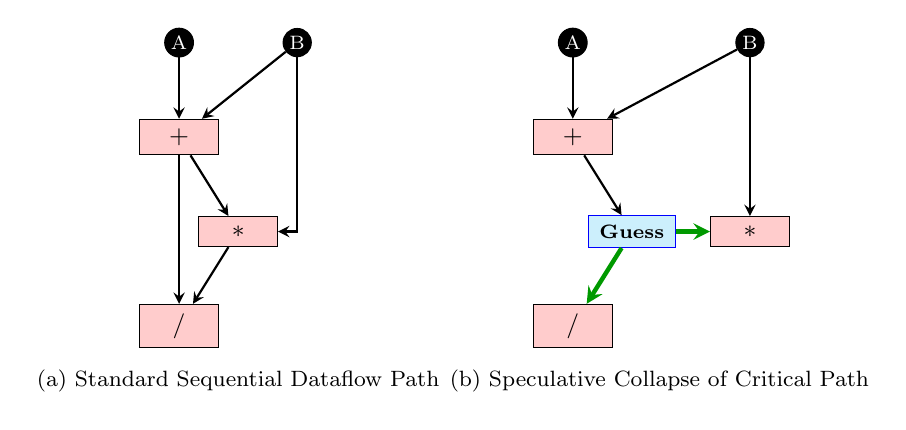
\begin{tikzpicture}[node distance=1.2cm, auto, >=stealth, font=\small]
    % Left Graph: Non-speculative
    \node [circle, draw, fill=black, text=white, inner sep=1pt] (a1) at (-3.5, 4.0) {\scriptsize A};
    \node [circle, draw, fill=black, text=white, inner sep=1pt] (b1) at (-2.0, 4.0) {\scriptsize B};
    
    \node [draw, rectangle, fill=red!20, minimum width=1.0cm] (add1) at (-3.5, 2.8) {$+$};
    \node [draw, rectangle, fill=red!20, minimum width=1.0cm] (mul1) at (-2.75, 1.6) {$*$};
    \node [draw, rectangle, fill=red!20, minimum width=1.0cm] (div1) at (-3.5, 0.4) {$/$};

    \draw [->, thick] (a1) -- (add1);
    \draw [->, thick] (b1) -- (add1);
    \draw [->, thick] (add1) -- (mul1);
    \draw [->, thick] (b1) |- (mul1);
    \draw [->, thick] (mul1) -- (div1);
    \draw [->, thick] (add1) -- (div1);

    \node at (-2.75, -0.3) {\footnotesize (a) Standard Sequential Dataflow Path};

    % Right Graph: Speculative Guessing
    \node [circle, draw, fill=black, text=white, inner sep=1pt] (a2) at (1.5, 4.0) {\scriptsize A};
    \node [circle, draw, fill=black, text=white, inner sep=1pt] (b2) at (3.75, 4.0) {\scriptsize B};
    
    \node [draw, rectangle, fill=red!20, minimum width=1.0cm] (add2) at (1.5, 2.8) {$+$};
    \node [draw, rectangle, fill=cyan!20, draw=blue, minimum width=1.1cm, font=\scriptsize\bfseries] (guess) at (2.25, 1.6) {Guess};
    \node [draw, rectangle, fill=red!20, minimum width=1.0cm] (mul2) at (3.75, 1.6) {$*$};
    \node [draw, rectangle, fill=red!20, minimum width=1.0cm] (div2) at (1.5, 0.4) {$/$};

    \draw [->, thick] (a2) -- (add2);
    \draw [->, thick] (b2) -- (add2);
    \draw [->, thick, green!60!black, ultra thick] (guess) -- (mul2);
    \draw [->, thick, green!60!black, ultra thick] (guess) -- (div2);
    \draw [->, thick] (b2) -- (mul2);
    \draw [->, thick] (add2) -- (guess);

    \node at (2.6, -0.3) {\footnotesize (b) Speculative Collapse of Critical Path};
\end{tikzpicture}
\caption{Comparison of execution graphs: standard sequential dataflow path vs. speculatively guessing data values to execute dependent operations in parallel.}
\label{fig:dataflow_value_speculation}
\end{figure}

\begin{concept}{Dataflow Critical Path Collapsing}{critical-path-collapsing}
By predicting intermediate calculation values:
\begin{itemize}
    \item \textbf{Standard Dataflow Graph:} Downstream operations ($*, /$) must wait sequentially for predecessor instructions ($+$) to complete execution, enforcing serial execution latency along the critical path.
    \item \textbf{Speculative Dataflow Graph:} A predictor introduces a speculative ``Guess'' value. Downstream instructions execute in parallel with the long-latency predecessor. Once the predecessor completes, the guess is verified; if correct, critical path latency is reduced to parallel execution depth.
\end{itemize}
\end{concept}

\subsection{Taxonomy of Data Value Patterns}
\label{subsec:value_pattern_taxonomy}

In their landmark study (\textit{``The Predictability of Data Values''}, MICRO-30, 1997), Yiannakis Sazeides and James Smith established that runtime data values produced by instructions exhibit structured, repetitive patterns.

\begin{definition}{Data Value Pattern Taxonomy}{data-value-patterns}
Instruction execution value sequences are categorized into five fundamental behavioral patterns:
\begin{itemize}
    \item \textbf{Constant ($C$):} The instruction produces the exact same value across consecutive executions:
    \[
    5, 5, 5, 5, 5, 5, \dots
    \]
    \item \textbf{Stride ($S$):} The value changes by a constant additive stride $\Delta = v_n - v_{n-1}$:
    \[
    1, 2, 3, 4, 5, 6, \dots \quad (\Delta = +1)
    \]
    \item \textbf{Non-Stride ($NS$):} Values change dynamically without any fixed arithmetic difference between consecutive steps:
    \[
    28, 13, 99, 107, 23, 456, \dots
    \]
    \item \textbf{Repeated Stride ($RS$):} Sequences composed of repeating sub-sequences governed by stride patterns:
    \[
    1, 2, 3, \quad 1, 2, 3, \quad 1, 2, 3, \dots
    \]
    \item \textbf{Repeated Non-Stride ($RNS$):} Repeating sequences of arbitrary values that exhibit no uniform additive stride:
    \[
    1, 13, 99, 7, \quad 1, 13, 99, 7, \dots
    \]
\end{itemize}
\end{definition}

To capture these patterns, data value predictors are partitioned into two algorithmic classes: \textbf{Computational Predictors} and \textbf{Context-Based Predictors}.

\subsection{Computational Value Predictors}
\label{subsec:computational_predictors}

\begin{concept}{Computational Predictors}{computational-predictors}
Computational predictors compute the predicted value as a deterministic mathematical function $\hat{v}_n = f(v_{n-1}, v_{n-2}, \dots)$ of previous instruction outputs.
\end{concept}

\subsubsection{Last-Value Predictors}
A Last-Value Predictor guesses that an instruction will reproduce its most recently observed execution output ($\hat{v}_n = v_{n-1}$).

To prevent temporary phase transitions or isolated mispredictions from polluting the prediction table, updating the stored value requires \textbf{hysteresis}:
\begin{itemize}
    \item \textbf{Saturating Counter Scheme:} Each table entry maintains a saturating confidence counter. The counter increments on prediction success and decrements on failure. The stored value is overwritten with a newly observed value only when the counter falls below a predefined threshold.
    \item \textbf{Observation Frequency Scheme:} Tracks how many times a newly observed value recurs consecutively. The stored prediction value is updated only after the new value is observed frequently enough (exceeding a confidence threshold).
\end{itemize}

\subsubsection{Stride Predictors}
Stride Predictors predict the next value by adding the most recent stride $\Delta = v_{n-1} - v_{n-2}$ to the latest observed value $v_{n-1}$:
\begin{equation}
\hat{v}_n = v_{n-1} + (v_{n-1} - v_{n-2})
\end{equation}

To avoid updating the stride on temporary loop control perturbations, hysteresis mechanisms are integrated:
\begin{itemize}
    \item \textbf{Saturating Counter Hysteresis:} The active stride is updated only when confidence counters drop below a failure threshold.
    \item \textbf{Two-Delta Stride Method:} Maintains two separate stride state variables per entry ($S_1$ and $S_2$):
    \begin{itemize}
        \item $S_1$ is continuously updated with the raw difference between the two most recent values ($v_{n-1} - v_{n-2}$).
        \item $S_2$ is the active stride used to compute predictions ($\hat{v}_n = v_{n-1} + S_2$).
        \item $S_2$ is updated to match $S_1$ ($S_1 \to S_2$) only when $S_1$ is observed twice in succession, preventing single-iteration loop boundaries from causing mispredictions.
    \end{itemize}
\end{itemize}

\subsection{Context-Based Value Predictors}
\label{subsec:context_based_predictors}

\begin{concept}{Context-Based Predictors}{context-based-predictors}
Context-Based Predictors learn the value that empirically follows a specific historical sequence (or context) of prior values, without assuming any mathematical functional relationship (e.g., linear strides).
\end{concept}

\subsubsection{Finite Context Method (FCM) Predictor}
The \gls{fcm} predictor records value transition frequencies based on a history of $k$ preceding unique values (referred to as an \textit{Order-$k$} predictor):
\begin{itemize}
    \item \textbf{Order-0 Predictor:} Purely frequency-based; predicts the value that has occurred most frequently over the entire execution history of the instruction.
    \item \textbf{Order-$k$ Predictor ($k \ge 1$):} Uses a hash of the last $k$ values as a lookup key into a history table that outputs the most likely succeeding value.
\end{itemize}

FCM predictors excel at capturing complex non-linear patterns, such as Repeated Stride ($RS$) and Repeated Non-Stride ($RNS$) sequences, which fail under linear computational stride predictors.

\subsection{Empirical Comparison of Value Predictors}
\label{subsec:empirical_predictor_comparison}

Sazeides and Smith evaluated the relative prediction coverage of distinct value predictors over benchmark execution traces using four classification categories:
\begin{itemize}
    \item \textbf{$np$:} Not predicted by any model.
    \item \textbf{$l$:} Correctly predicted by Last-Value predictors.
    \item \textbf{$s$:} Correctly predicted by Stride predictors (Two-Delta).
    \item \textbf{$f$:} Correctly predicted by Context-based predictors (Order-3 FCM).
\end{itemize}

\begin{observation}{Empirical Predictability of Data Values}{empirical-value-predictability}
Comparative evaluation reveals key insights into data value predictability across application workloads:
\begin{itemize}
    \item \textbf{Universal Predictability:} Approximately \textbf{40\%} of all generated data values are correctly predicted by all predictor types ($l, s, f$), reflecting the high prevalence of constant ($C$) values.
    \item \textbf{Exclusive Context Coverage:} Approximately \textbf{20\%} of values are captured exclusively by Order-3 FCM context predictors ($f$). Computational stride and last-value predictors fail on these sequences because the values lack linear arithmetic relationships.
    \item \textbf{Unpredictable Baseline:} Only \textbf{18\%} of runtime data values are completely unpredictable ($np$) across all models.
    \item \textbf{Computational Predictor Limits:} Stride ($s$) and Last-Value ($l$) predictors combined capture less than \textbf{5\%} of correct predictions missed by FCM, proving that context-based models subsume nearly all predictable computational structures.
\end{itemize}
\end{observation}

\section{Superscalar Architectures}
\label{sec:superscalar_architectures}

To break the theoretical execution boundary of scalar processors ($\text{CPI} = 1$) and achieve a Cycles Per Instruction $\text{CPI} < 1$ (or equivalently, an Instructions Per Cycle $\text{IPC} > 1$), microarchitectures must fetch, decode, issue, and execute multiple instructions simultaneously within every clock cycle.

\begin{definition}{Superscalar vs. VLIW Architectures}{superscalar-vs-vliw}
Architectures capable of executing multiple instructions per cycle fall into two structural paradigms based on whether instruction scheduling is performed dynamically by hardware or statically by the compiler:
\begin{itemize}
    \item \textbf{Superscalar Architecture:} Hardware dynamically fetches, decodes, and schedules a variable number of instructions per clock cycle based on runtime resource availability and data dependencies.
    \item \textbf{Very Long Instruction Word (VLIW):} The compiler statically packs a fixed number of independent operations (typically 4 to 16) into a single wide instruction template. The hardware executes these operations in parallel without performing dynamic dependency checks.
\end{itemize}
\end{definition}

The adoption of multi-issue architectures led to a shift in performance metrics, making \textbf{Instructions Per Clock Cycle (IPC)} the primary metric of processing throughput rather than traditional CPI.

\section{Superscalar Issue Mechanics and Parameters}
\label{sec:superscalar_issue_mechanics}

The core structural challenge of superscalar execution lies in managing the enlarged \textbf{instruction window} and checking dependencies across multiple candidate instructions concurrently.

\begin{concept}{Superscalar Issue Parameters and Policies}{superscalar-issue-policies}
Superscalar issue performance is defined by three fundamental parameters:
\begin{enumerate}
    \item \textbf{Instruction Window:} The set of instructions residing in the instruction buffer/queue that are evaluated simultaneously by hardware for potential issue.
    \item \textbf{Issue Width (Issue Rate):} The maximum number of instructions that can be dispatched from the issue window to execution buffers in a single clock cycle.
    \item \textbf{Issue Policy:} Defines how the processor handles data and structural dependencies during instruction dispatch:
    \begin{itemize}
        \item \textbf{Blocking Issue (In-Order Issue):} Instructions are held in the issue window until all dependencies are resolved. If an instruction at the head of the window stalls due to a hazard, all subsequent instructions in the issue window are blocked from issuing.
        \item \textbf{Non-Blocking Issue (Shelving / Out-of-Order Issue):} Instructions are dispatched from the issue window into intermediate reservation stations or shelving buffers regardless of pending data hazards. Dependency checking is decoupled from the issue stage and performed at dispatch/execution.
    \end{itemize}
\end{enumerate}
\end{concept}

\subsection{Pipelining the Decode and Issue Stages}
In a scalar processor, only one instruction is decoded and issued per cycle, requiring dependency checks strictly between the single candidate instruction and in-flight execution units. 

In a superscalar processor with issue width $N$:
\begin{itemize}
    \item \textbf{Intra-Window Dependency Checks:} The hardware must perform $\mathcal{O}(N^2)$ parallel comparisons to check dependencies \textit{among} the $N$ candidate instructions decoded within the current cycle's issue window.
    \item \textbf{Inter-Window Dependency Checks:} The hardware must simultaneously check dependencies between the $N$ candidate instructions and all in-flight instructions currently executing or shelved in reservation stations.
\end{itemize}

Because of the massive quadratic growth in logic gate complexity required for multi-instruction hazard detection, high-performance microarchitectures routinely split the Decode and Issue phases into multiple pipelined stages.

\section{Integrated Instruction Fetch Unit (IIFU)}
\label{sec:iifu}

To keep multi-issue execution pipelines saturated, the front-end must supply a continuous stream of instructions at a rate equal to or exceeding the maximum issue width. This is managed by an \textbf{Integrated Instruction Fetch Unit (IIFU)}.

\begin{concept}{Integrated Instruction Fetch Unit (IIFU)}{iifu-concept}
The IIFU decouples memory access bottlenecks from front-end execution by integrating three key components:
\begin{itemize}
    \item \textbf{High-Throughput Branch Predictor:} Predicts branch outcomes and target addresses speculatively to maintain an uninterrupted instruction stream across control flow boundaries.
    \item \textbf{Instruction Prefetch Unit:} Fetches instructions ahead of program execution from lower memory levels into high-speed buffers to hide cache miss latencies.
    \item \textbf{I-Cache Access and Buffering Engine:} Manages multi-word instruction fetches from the L1 Instruction Cache. When a fetched block spans across L1 cache line boundaries or memory blocks, the IIFU buffers and aligns the stream before forwarding it to the instruction window.
\end{itemize}
\end{concept}

\section{Predecoding Techniques}
\label{sec:predecoding}

Decoding complex instructions or identifying instruction boundaries in multi-issue front-ends creates a significant latency bottleneck during the Decode phase. To mitigate this, superscalar processors implement \textbf{Predecoding}.

\begin{observation}{Predecoding Mechanisms}{predecoding-mechanisms}
Predecoding shifts part of the instruction decoding workload from the critical execution path into the L1 Instruction Cache loading phase:
\begin{itemize}
    \item When instructions are loaded from lower-level memory (L2/L3 cache or main memory) into the on-chip L1 Instruction Cache, a predecode unit analyzes the raw bytes and appends extra \textbf{predecode bits} (tags) to each cached instruction.
    \item \textbf{Predecode Information:} The added predecode bits explicitly store:
    \begin{itemize}
        \item The basic instruction class and opcode category (e.g., branch, load/store, integer ALU, floating-point).
        \item The specific functional unit resources required for execution.
        \item Pre-calculated branch target displacements or static branch properties.
    \end{itemize}
    \item \textbf{CISC Variable-Length Decoding:} For CISC architectures with variable-length instruction encodings (such as x86), predecoding identifies the exact start and end byte boundaries of consecutive instructions. This enables the parallel decode unit to immediately slice the instruction byte stream into valid instruction blocks without sequential parsing stalls.
\end{itemize}
\end{observation}

\section{Loop Unrolling in Superscalar Architectures}
\label{sec:loop_unrolling_superscalar}

Loop unrolling is a fundamental transformation technique designed to expose \glsfmtshort{ilp} by replicating a loop body multiple times and reducing control overhead. In superscalar processors, combining loop unrolling with hardware speculation yields dramatic throughput gains compared to non-speculative execution.

\begin{concept}{Loop Unrolling Mechanics}{loop-unrolling-concept}
Loop unrolling increases instruction throughput by:
\begin{itemize}
    \item \textbf{Amortizing Control Overhead:} Decreasing the frequency of branch evaluations and loop counter updates relative to useful computation.
    \item \textbf{Expanding the Scheduling Window:} Providing a larger pool of independent instructions for multi-issue dispatch.
    \item \textbf{Eliminating False Dependencies:} Re-allocating destination registers across unrolled iterations to remove \glsfmtshort{waw} and \glsfmtshort{war} name hazards.
\end{itemize}
\end{concept}

\subsection{Superscalar Loop Execution Without Speculation}
\label{subsec:unrolling_without_speculation}

Consider a loop updating an array of 64-bit floating-point values ($x[i] = x[i] + \text{scalar}$). In a dual-issue superscalar pipeline (Slot 1: Memory/Integer ALU; Slot 2: Floating-Point ALU) operating \textbf{without speculation}, the compiler must unroll the loop statically (e.g., $4\times$) and interleave independent operations using distinct architectural registers ($F_0, F_6, F_{10}, F_{14}$).

\begin{lstlisting}[language=C, caption={$4\times$ Unrolled Loop without Speculation}]
Loop: L.D    F0, 0(R1)       ; Iteration 1 Load
      L.D    F6, -8(R1)      ; Iteration 2 Load
      L.D    F10, -16(R1)    ; Iteration 3 Load
      L.D    F14, -24(R1)    ; Iteration 4 Load
      ADD.D  F4, F0, F2      ; Iteration 1 Add
      ADD.D  F8, F6, F2      ; Iteration 2 Add
      ADD.D  F12, F10, F2    ; Iteration 3 Add
      ADD.D  F16, F14, F2    ; Iteration 4 Add
      S.D    F4, 0(R1)       ; Iteration 1 Store
      S.D    F8, -8(R1)      ; Iteration 2 Store
      S.D    F12, -16(R1)    ; Iteration 3 Store
      S.D    F16, -24(R1)    ; Iteration 4 Store
      DADDUI R1, R1, #-32    ; Decrement pointer by 32 bytes (4 * 8)
      BNE    R1, R2, Loop    ; Non-speculative branch barrier
\end{lstlisting}

\begin{table}[htbp]
\centering
\caption{Dual-Issue Pipeline Schedule: $4\times$ Unrolled Loop Without Speculation}
\label{tab:schedule_no_speculation}
\small
\setlength{\tabcolsep}{4pt}
\begin{tabularx}{\textwidth}{|c|>{\hsize=1.1\hsize\raggedright\arraybackslash}X|>{\hsize=1.1\hsize\raggedright\arraybackslash}X|>{\hsize=0.8\hsize\raggedright\arraybackslash}X|}
\hline
\textbf{Clock Cycle} & \textbf{ALU / Memory Slot} & \textbf{FP Instruction Slot} & \textbf{Pipeline Status} \\ \hline
\textbf{CC 1} & \texttt{L.D F0, 0(R1)} & \textit{stall} & Issue Iter 1 Load \\ \hline
\textbf{CC 2} & \texttt{L.D F6, -8(R1)} & \textit{stall} & Issue Iter 2 Load \\ \hline
\textbf{CC 3} & \texttt{L.D F10, -16(R1)} & \texttt{ADD.D F4, F0, F2} & F0 ready; Issue Iter 3 Load \& Iter 1 Add \\ \hline
\textbf{CC 4} & \texttt{L.D F14, -24(R1)} & \texttt{ADD.D F8, F6, F2} & F6 ready; Issue Iter 4 Load \& Iter 2 Add \\ \hline
\textbf{CC 5} & \textit{stall} & \texttt{ADD.D F12, F10, F2} & F10 ready; Issue Iter 3 Add \\ \hline
\textbf{CC 6} & \texttt{S.D F4, 0(R1)} & \texttt{ADD.D F16, F14, F2} & F4 ready; Store Iter 1 \& Issue Iter 4 Add \\ \hline
\textbf{CC 7} & \texttt{S.D F8, -8(R1)} & \textit{stall} & F8 ready; Store Iter 2 \\ \hline
\textbf{CC 8} & \texttt{S.D F12, -16(R1)} & \textit{stall} & Store Iter 3 \\ \hline
\textbf{CC 9} & \texttt{S.D F16, -24(R1)} & \textit{stall} & Store Iter 4 \\ \hline
\textbf{CC 10} & \texttt{DADDUI R1, R1, \#-32} & \textit{stall} & Pointer Update \\ \hline
\textbf{CC 11} & \texttt{BNE R1, R2, Loop} & \textit{stall} & \textbf{Branch Hazard Stall} (Wait for resolution) \\ \hline
\end{tabularx}
\end{table}

\begin{observation}{Limitations of Non-Speculative Loop Unrolling}{limits-no-speculation}
Without hardware speculation:
\begin{enumerate}
    \item \textbf{Register Pressure:} Statically allocating separate registers ($F_0, F_6, F_{10}, F_{14}$) rapidly exhausts the architectural register file.
    \item \textbf{Branch Control Barriers:} Issue stalls at the terminating branch (\texttt{BNE}) at cycle 11, preventing instructions from iteration $N+1$ from entering the pipeline.
    \item \textbf{Instruction Cache Inflation:} Code replication bloats the L1 Instruction Cache footprint.
\end{enumerate}
\end{observation}

\subsection{Superscalar Loop Execution With Hardware Speculation}
\label{subsec:unrolling_with_speculation}

Combining loop unrolling with hardware speculation (via Branch Prediction, Reorder Buffer, and Explicit/Implicit Register Renaming) eliminates static code bloat and branch barriers.

\begin{concept}{Dynamic Speculative Loop Execution}{speculative-loop-execution}
Under hardware speculation:
\begin{itemize}
    \item \textbf{Branch Bypassing:} The branch predictor predicts loop branches continuously, allowing the fetch engine to stream subsequent loop iterations into the pipeline without stalling.
    \item \textbf{Dynamic Hardware Renaming:} The Physical Register File (\glsfmtshort{prf}) and Register Alias Table (\glsfmtshort{rat}) automatically map repeated architectural register names ($F_0$) to fresh physical tags ($P_{16}, P_{18}, P_{20}, \dots$), resolving \glsfmtshort{waw} and \glsfmtshort{war} hazards dynamically.
    \item \textbf{Speculative Memory Disambiguation:} The Speculative Store Buffer (\glsfmtshort{ssb}) holds store payloads safely until commit, enabling loads from iteration $N+1$ to execute speculatively ahead of stores from iteration $N$.
\end{itemize}
\end{concept}

\begin{table}[htbp]
\centering
\caption{Dynamic Speculative Trace of Baseline Single-Body Loop across Multiple Iterations}
\label{tab:speculative_loop_trace}
\small
\setlength{\tabcolsep}{3pt}
\begin{tabularx}{\textwidth}{|c|>{\hsize=0.6\hsize\raggedright\arraybackslash}X|>{\hsize=1.1\hsize\raggedright\arraybackslash}X|>{\hsize=1.1\hsize\raggedright\arraybackslash}X|>{\hsize=1.2\hsize\raggedright\arraybackslash}X|}
\hline
\textbf{Iter} & \textbf{Instruction} & \textbf{Rename Mapping (\glsfmtshort{rat})} & \textbf{\glsfmtshort{rob} Entry} & \textbf{Commit Order (In-Order)} \\ \hline
\textbf{1} & \texttt{L.D F0, 0(R1)} & $F_0 \to P_{16}$ & $\text{\glsfmtshort{rob}}_1$ (Speculative) & Commits 1st (Writes L1 on commit) \\
\textbf{1} & \texttt{ADD.D F4, F0, F2} & $F_4 \to P_{17}$ (reads $P_{16}$) & $\text{\glsfmtshort{rob}}_2$ (Speculative) & Commits 2nd \\
\textbf{1} & \texttt{S.D F4, 0(R1)} & Reads $P_{17}$ & $\text{\glsfmtshort{rob}}_3$ (Buffered in SSB) & Commits 3rd (Flushes SSB to L1) \\
\textbf{1} & \texttt{BNE R1, R2} & Predicted \textit{Taken} & $\text{\glsfmtshort{rob}}_4$ (Speculative) & Commits 4th (Branch verified) \\ \hline
\textbf{2} & \texttt{L.D F0, -8(R1)} & $F_0 \to P_{18}$ (\textbf{No WAW}) & $\text{\glsfmtshort{rob}}_5$ (Speculative) & Commits 5th \\
\textbf{2} & \texttt{ADD.D F4, F0, F2} & $F_4 \to P_{19}$ (reads $P_{18}$) & $\text{\glsfmtshort{rob}}_6$ (Speculative) & Commits 6th \\
\textbf{2} & \texttt{S.D F4, -8(R1)} & Reads $P_{19}$ & $\text{\glsfmtshort{rob}}_7$ (Buffered in SSB) & Commits 7th \\
\textbf{2} & \texttt{BNE R1, R2} & Predicted \textit{Taken} & $\text{\glsfmtshort{rob}}_8$ (Speculative) & Commits 8th \\ \hline
\textbf{3} & \texttt{L.D F0, -16(R1)} & $F_0 \to P_{20}$ (\textbf{No WAW}) & $\text{\glsfmtshort{rob}}_9$ (Speculative) & Commits 9th \\
\textbf{3} & \texttt{ADD.D F4, F0, F2} & $F_4 \to P_{21}$ (reads $P_{20}$) & $\text{\glsfmtshort{rob}}_{10}$ (Speculative) & Commits 10th \\
\hline
\end{tabularx}
\end{table}

\begin{table}[htbp]
\centering
\caption{Architectural Comparison of Loop Unrolling Paradigms}
\label{tab:unrolling_comparison_summary}
\small
\setlength{\tabcolsep}{4pt}
\begin{tabularx}{\textwidth}{|>{\hsize=0.8\hsize\raggedright\arraybackslash}X|>{\hsize=1.1\hsize\raggedright\arraybackslash}X|>{\hsize=1.1\hsize\raggedright\arraybackslash}X|}
\hline
\textbf{Feature / Dimension} & \textbf{Unrolling Without Speculation} & \textbf{Unrolling With Hardware Speculation} \\ \hline
\textbf{Unrolling Mechanism} & Static compiler transformation & Dynamic hardware unrolling across \glsfmtshort{rob} \\ \hline
\textbf{Register Allocation} & Consumes multiple \glsfmtshort{isa} architectural registers ($F_0, F_6, F_{10}$) & Uses single \glsfmtshort{isa} register ($F_0$), mapped dynamically to Physical Registers ($P_{16}, P_{18}, P_{20}$) \\ \hline
\textbf{Branch Handling} & Issue stalls at unrolled block terminating branches & Zero-stall branch prediction; fetches across branch boundaries \\ \hline
\textbf{Memory Scheduling} & Strict non-speculative memory order; load/store reordering restricted & Speculative Store Buffer (\glsfmtshort{ssb}) enables early load execution via store-to-load forwarding \\ \hline
\textbf{Binary Code Size} & Multiplied by unroll factor ($N\times$ code size expansion) & Compact baseline code size; zero instruction cache bloat \\ \hline
\textbf{Exception Handling} & Potential imprecise exceptions if instructions are reordered statically & Precise exceptions guaranteed by in-order \glsfmtshort{rob} retirement \\ \hline
\end{tabularx}
\end{table}

\section{Challenges in Multiple-Issue Architectures}
\label{sec:multiple_issue_challenges}

While expanding execution width from scalar to superscalar promises ideal throughput scaling ($\text{IPC} = N$), real-world microarchitectures face severe structural and algorithmic bottlenecks.

\begin{observation}{Limitations of Static Dual-Issue Pipelines}{static-dual-issue-limits}
A simple split-functional unit dual-issue processor (issuing 1 Integer/Memory operation + 1 Floating-Point operation per cycle) achieves its theoretical peak of $\text{CPI} = 0.5$ ($\text{IPC} = 2.0$) \textbf{only under two restrictive conditions}:
\begin{enumerate}
    \item The instruction stream contains an \textbf{exact 50\% / 50\% split} between Integer and Floating-Point operations.
    \item There are \textbf{zero data or structural hazards} between concurrently issued instructions.
\end{enumerate}
In general workloads, asymmetric instruction mixes and inter-instruction dependencies severely degrade actual IPC.
\end{observation}

\subsection{Combinatorial Complexity of Wide Decoding and Issue}
As issue width $N$ grows, the hardware complexity of the Decode and Issue stages increases quadratically ($\mathcal{O}(N^2)$):
\begin{itemize}
    \item \textbf{Opcode and Specifier Inspection:} A 2-scalar processor must simultaneously inspect 2 opcodes, extract 6 register specifiers (2 destinations, 4 sources), and evaluate dependency logic within a single clock cycle.
    \item \textbf{Multiported Register Files and Rename Tables:} To issue $N$ instructions per cycle, the Register Alias Table (\glsfmtshort{rat}) and Physical Register File (\glsfmtshort{prf}) must support up to $2N$ read ports and $N$ write ports.
    \item \textbf{Multi-Instruction Rename Logic:} The rename unit must be capable of allocating physical registers and updating mapping tables for multiple instructions in parallel—including handling dependency chains \textit{within} the same issue packet.
\end{itemize}

\subsection{Very Long Instruction Word (VLIW) Trade-Offs}
To avoid complex dynamic multi-issue hardware, \textbf{VLIW (Very Long Instruction Word)} architectures shift scheduling entirely to the compiler.

\begin{concept}{VLIW Trade-Offs}{vliw-tradeoffs}
VLIW trades instruction memory space for simple hardware decoding:
\begin{itemize}
    \item \textbf{Fixed Wide Templates:} The compiler packs multiple independent operations into a single wide instruction template (typically 112 to 168 bits wide, containing 4 to 8 execution slots).
    \item \textbf{Hardware Simplicity:} Because the compiler guarantees that all operations within a VLIW word are independent, the hardware executes them in parallel without dynamic dependency checking logic.
    \item \textbf{Compiler Requirement:} Requires advanced global compilation techniques (such as Trace Scheduling or Software Pipelining) to find independent operations across multiple branch boundaries.
\end{itemize}
\end{concept}

\section{Superscalar Dynamic Register Renaming}
\label{sec:superscalar_register_renaming}

In a superscalar processor, renaming multiple instructions simultaneously per clock cycle introduces a critical hazard: \textbf{Intra-Cycle Read-After-Write (RAW) Dependencies}.

\subsection{Naive Parallel Renaming (Try \#1: Independent Lookup Failure)}

Consider a dual-issue front-end attempting to rename two instructions ($\text{Inst}_1$ and $\text{Inst}_2$) in parallel during the same clock cycle:
\begin{align*}
\text{Inst}_1&: \quad R_d^1 \leftarrow R_{s1}^1 \text{ op } R_{s2}^1 \\
\text{Inst}_2&: \quad R_d^2 \leftarrow R_{s1}^2 \text{ op } R_{s2}^2
\end{align*}

In a naive parallel rename implementation (Try \#1):
\begin{enumerate}
    \item Both instructions send their source register specifiers ($R_{s1}^1, R_{s2}^1$ and $R_{s1}^2, R_{s2}^2$) to the Rename Table simultaneously.
    \item The Free List allocates two physical registers ($P_{\text{dest}}^1$ and $P_{\text{dest}}^2$).
    \item The Rename Table updates its entries for $R_d^1$ and $R_d^2$ with $P_{\text{dest}}^1$ and $P_{\text{dest}}^2$.
\end{enumerate}

\begin{observation}{Failure Mode of Try \#1 (Intra-Cycle RAW Hazard)}{try1-failure}
If $\text{Inst}_2$ reads an architectural register written by $\text{Inst}_1$ in the same cycle ($R_{s1}^2 == R_d^1$), naive parallel lookup fails: $\text{Inst}_2$ reads the \textbf{old} physical register mapping for $R_d^1$ from the Rename Table because $\text{Inst}_1$'s new mapping ($P_{\text{dest}}^1$) has not yet been written back to the table!
\end{observation}

\subsection{Intra-Cycle RAW Hazard Detection and Bypass (Try \#2)}

To resolve intra-cycle dependencies, superscalar rename units integrate \textbf{intra-cycle comparator and bypass logic} (Try \#2).

\begin{definition}{Intra-Cycle RAW Hazard Bypass}{try2-definition}
In Try \#2 superscalar renaming, the rename logic performs parallel equality checks ($=?$) between the destination register of earlier instructions and the source registers of later instructions issued in the same cycle:
\begin{equation}
\text{Match}_{s1} = (R_d^1 == R_{s1}^2), \quad \text{Match}_{s2} = (R_d^1 == R_{s2}^2)
\end{equation}
If a match is detected ($\text{Match} = \text{true}$), a multiplexer bypasses the Rename Table lookup output for $\text{Inst}_2$'s source, replacing it directly with $\text{Inst}_1$'s newly allocated physical destination register ($P_{\text{dest}}^1$).
\end{definition}

\begin{figure}[htpb]
\centering
\begin{tikzpicture}[
    scale=0.9,
    >=Stealth,
    font=\sffamily\small,
    box/.style={
        draw=black!70, 
        fill=white, 
        rounded corners=4pt, 
        thick, 
        inner sep=6pt, 
        align=center
    },
    inst/.style={
        box, 
        fill=gray!10, 
        minimum width=5.2cm, 
        font=\scriptsize
    },
    block/.style={
        box, 
        minimum height=1.3cm
    },
    comp/.style={
        circle, 
        draw=orange!80!black, 
        fill=orange!25, 
        thick, 
        inner sep=0pt, 
        font=\bfseries\tiny, 
        minimum size=7mm
    },
    mux/.style={
        box, 
        fill=yellow!35, 
        draw=yellow!60!black, 
        font=\bfseries\tiny, 
        minimum width=1.5cm, 
        minimum height=0.6cm
    },
    outbox/.style={
        box, 
        fill=blue!8, 
        draw=blue!40!black, 
        minimum width=5.4cm, 
        font=\scriptsize
    },
    line/.style={draw=gray!80!black, thick, ->},
    data/.style={draw=red!70!black, thick, ->},
    free/.style={draw=green!60!black, thick, ->},
    ctrl/.style={draw=gray!60, thick, dashed, ->}
]

    % --- 1. NODI PRINCIPALI ---
    \node [inst] (inst1) at (-4.5, 5.5) {%
        \textbf{Inst 1:} \texttt{[Op | Dest1 | Src1\_1 | Src2\_1]}
    };
    \node [inst] (inst2) at (4.5, 5.5) {%
        \textbf{Inst 2:} \texttt{[Op | Dest2 | Src1\_2 | Src2\_2]}
    };

    \node [block, fill=blue!12, draw=blue!50!black, minimum width=4.4cm] (rat) at (-4.5, 3.0) {%
        \textbf{Rename Table (RAT)}\\[2pt]\tiny 4 Read Ports / 2 Write Ports
    };
    \node [block, fill=green!12, draw=green!50!black, minimum width=4.2cm] (free_list) at (4.5, 3.0) {%
        \textbf{Register Free List}\\[2pt]\tiny Allocates $PDest_1, PDest_2$
    };

    \node [comp] (comp1) at (-1.2, 0.4) {=?};
    \node [comp] (comp2) at (1.2, 0.4) {=?};

    \node [mux] (mux1) at (-1.2, -1.8) {MUX 1};
    \node [mux] (mux2) at (1.2, -1.8) {MUX 2};

    \node [outbox] (out1) at (-4.5, -4.5) {%
        \textbf{Renamed Inst 1:}\\[2pt]\texttt{[Op | PDest1 | PSrc1\_1 | PSrc2\_1]}
    };
    \node [outbox] (out2) at (4.5, -4.5) {%
        \textbf{Renamed Inst 2:}\\[2pt]\texttt{[Op | PDest2 | PSrc1\_2 | PSrc2\_2]}
    };


    % --- 2. COLLEGAMENTI SU GRIGLIA ASSOLUTA ---

    % Sorgenti -> RAT (Percorso pulito a 90 gradi sopra la RAT)
    \draw [line] (inst1.south) -- (rat.north);
    \draw [line] (inst2.south) -- ++(0,-0.6) -- (-2.2, 4.9) -- (-2.2, 3.65);

    % Linea Rossa Dest1 -> Comparatori
    \draw [data] (-3.8, 5.15) -- (-3.8, 4.4) -- (0.0, 4.4) -- (0.0, 1.4) coordinate (red_node);
    \draw [data] (red_node) -| (comp1.north) node[pos=0.1, above left, font=\tiny\bfseries] {$Dest_1$};
    \draw [data] (red_node) -| (comp2.north);

    % Sorgenti Inst 2 -> Comparatori (Canale di Destra)
    \draw [line] (3.8, 5.15) -- (3.8, 0.4) -- (comp2.east) 
        node[pos=0.7, above, font=\tiny] {$Src2_2\ $};
    \draw [line] (4.8, 5.15) -- (4.8, -0.2) -- (2.6, -0.2) -- (2.6, 0.4) -- (comp1.east |- 0, 0.4)
        node[pos=0.2, above, font=\tiny] {$Src1_2\ $};

    % Allocazione PDest1 (Linea verde: Free List -> Out1)
    \draw [free] (free_list.south) -- (4.5, 2.0) -- (-2.0, 2.0) -- (-2.0, -3.6) -- (-4.5, -3.6) -- (out1.north)
        node[pos=0.18, above, font=\tiny\bfseries] {$PDest_1$};

    % Allocazione PDest2 (Linea verde: Free List -> Out2)
    \draw [free] (6.0, 2.35) -- (6.0, -3.8) -- (4.5, -3.8) -- (out2.north)
        node[pos=0.5, right, font=\tiny\bfseries] {$PDest_2$};

    % Segnali di Controllo ai MUX
    \draw [ctrl] (comp1.south) -- (mux1.north);
    \draw [ctrl] (comp2.south) -- (mux2.north);

    % Bypass PDest1 ai MUX
    \draw [free] (-2.0, -0.9) -- (-0.2, -0.9) coordinate (b_node);
    \draw [free] (b_node) -| (mux1.north west) node[pos=0.1, above, font=\tiny\bfseries] {Bypass $PDest_1$};
    \draw [free] (b_node) -| (mux2.north west);

    % Output MUX -> Renamed Inst 2
    \draw [line] (mux1.south) -- (-1.2, -2.8) -- (3.8, -2.8) -- (3.8, -3.9) -- (out2.north -| 3.8, -3.9);
    \draw [line] (mux2.south) -- (1.2, -2.6) -- (4.8, -2.6) -- (4.8, -3.9) -- (out2.north -| 4.8, -3.9);

\end{tikzpicture}
\caption{Architecture of a Dual-Issue Superscalar Register Rename Unit with Intra-Cycle RAW Hazard Comparators and Bypass MUXes (Try \#2).}
\label{fig:superscalar_rename_try2}
\end{figure}

\begin{concept}{Case Study: MIPS R10000 (MIPS R10K)}{mips-r10k-renaming}
The \textbf{MIPS R10000} processor implemented a 4-issue superscalar pipeline capable of dynamically renaming up to \textbf{4 serially-RAW-dependent instructions within a single clock cycle}. 

To achieve this, the R10K rename logic contained a cascading matrix of 12 internal comparators that evaluated all pairwise combinations of destination and source register specifiers across the 4 candidate instructions in parallel, ensuring zero issue stalls even for tightly coupled execution sequences.
\end{concept}